%%%%%%%%%%%%%%%%%%%%%%%%%%%%%%%%%%%%%%%%%%%%%%%%%%%%%%%%%%%%%%%%%%%%%%%%%%%%%%%%
%2345678901234567890123456789012345678901234567890123456789012345678901234567890
%        1         2         3         4         5         6         7         8

\documentclass[letterpaper, 10 pt, conference]{ieeeconf}  % Comment this line out
                                                          % if you need a4paper
%\documentclass[a4paper, 10pt, conference]{ieeeconf}      % Use this line for a4
                                                          % paper

\IEEEoverridecommandlockouts                              % This command is only
                                                          % needed if you want to
                                                          % use the \thanks command
\overrideIEEEmargins
% See the \addtolength command later in the file to balance the column lengths
% on the last page of the document

% This is needed to prevent the style file preventing citations from linking to 
% the bibliography
\makeatletter
\let\NAT@parse\undefined
\makeatother

\usepackage[dvipsnames]{xcolor}

\newcommand*\linkcolours{ForestGreen}

\usepackage{times}
\usepackage{graphicx}
\usepackage{amssymb}
\usepackage{gensymb}
\usepackage{amsmath}
\usepackage{breakurl}
\def\UrlBreaks{\do\/\do-}
\usepackage{url,hyperref}
\hypersetup{
colorlinks,
linkcolor=\linkcolours,
citecolor=\linkcolours,
filecolor=\linkcolours,
urlcolor=\linkcolours}

\usepackage{algorithm}
\usepackage{algorithmic}

\usepackage[labelfont={bf},font=small]{caption}
\usepackage[none]{hyphenat}

\usepackage{mathtools, cuted}

\usepackage[noadjust, nobreak]{cite}
\def\citepunct{,\,} % Style file defaults to listing references separately

\usepackage{tabularx}
\usepackage{amsmath}

\usepackage{float}

\usepackage{pifont}% http://ctan.org/pkg/pifont
\newcommand{\cmark}{\ding{51}}%
\newcommand{\xmark}{\ding{55}}%

\newcommand*\diff{\mathop{}\!\mathrm{d}}
\newcommand*\Diff[1]{\mathop{}\!\mathrm{d^#1}}
\newcommand*\imgres{600}

\newcommand*\GitHubLoc{https://github.com/linted/allocation}

\newcolumntype{Y}{>{\centering\arraybackslash}X}

%\usepackage{parskip}

\usepackage[]{placeins}

\newcommand\extraspace{3pt}

\usepackage{placeins}

\usepackage{tikz}
\newcommand*\circled[1]{\tikz[baseline=(char.base)]{
            \node[shape=circle,draw,inner sep=0.8pt] (char) {#1};}}
            
\usepackage[framemethod=tikz]{mdframed}

\usepackage{afterpage}

\usepackage{stfloats}

\usepackage{atbegshi}
\newcommand{\handlethispage}{}
\newcommand{\discardpagesfromhere}{\let\handlethispage\AtBeginShipoutDiscard}
\newcommand{\keeppagesfromhere}{\let\handlethispage\relax}
\AtBeginShipout{\handlethispage}

\usepackage{comment}

\usepackage{listings}
% code box settings
\lstset{tabsize=4}
% \lstdefinelanguage
%    [x64]{Assembler}     % add a "x64" dialect of Assembler
%    [x86masm]{Assembler} % based on the "x86masm" dialect
%    % with these extra keywords:
%    {morekeywords={CDQE,CQO,CMPSQ,CMPXCHG16B,JRCXZ,LODSQ,MOVSXD, %
%                   POPFQ,PUSHFQ,SCASQ,STOSQ,IRETQ,RDTSCP,SWAPGS, %
%                   rax,rdx,rcx,rbx,rsi,rdi,rsp,rbp, %
%                   r8,r8d,r8w,r8b,r9,r9d,r9w,r9b, %
%                   r10,r10d,r10w,r10b,r11,r11d,r11w,r11b, %
%                   r12,r12d,r12w,r12b,r13,r13d,r13w,r13b, %
%                   r14,r14d,r14w,r14b,r15,r15d,r15w,r15b}} % etc.

\newcommand*\todo[0]{\textcolor{red}{TODO }}


\title{\LARGE \bf
Stack and Heap Allocations: A Cost Comparison
}


\author{Michael D. Merrill$^{1}$% <-this % stops a space
\thanks{$^{1}$Michael is a Masters student in Computer Sciences, Georgia Tech,
and a developer for the }%
}


\begin{document}


\maketitle
\thispagestyle{empty}
\pagestyle{empty}


%%%%%%%%%%%%%%%%%%%%%%%%%%%%%%%%%%%%%%%%%%%%%%%%%%%%%%%%%%%%%%%%%%%%%%%%%%%%%%%%
\begin{abstract}
Stack and Heap allocations have different allocation costs and use cases.
Incorrect choice of allocation method is often problematic and cause increases in latency,
loss of data, and program instability. I compare the choice of allocation method across various 
implementations and situations to show the cost benefit trade offs of each. 
Finally a quantitative explanation of the results through a high level description of the allocation algorithm internals is provided.
The source code is publicly available at \url{\GitHubLoc}.

\end{abstract}

%%%%%%%%%%%%%%%%%%%%%%%%%%%%%%%%%%%%%%%%%%%%%%%%%%%%%%%%%%%%%%%%%%%%%%%%%%%%%%%%
\section{INTRODUCTION}

Allocation algorithms are designed to limit the overhead related to memory management.
The most common design goals include considerations for computational expenses, effectiveness allocation size, and to provide discrete blocks of memory. 
Stack allocation on commonly used architectures, such as Intel x86, involve changing the value of a register to allocate additional space, and are thus standardized by the architecture.
Dynamic allocation, in contrast, is defined by userspace libraries.
This allows for multiple implementations of allocators, as well as specialized allocators which offer increased performance benefits for their use cases. 

This paper addresses the performance costs incurred through the use of the stack and heap across their various allocation methods. 
A number of test algorithms will be used as measurements. 
Each will attempt to measure a discrete feature and function common to all allocation algorithms. 
Care is taken to ensure that tests do not favor one method over another through intentional use of compiler hints and directives. 
The test algorithms are designed to mimic common, real world use cases of allocated memory as well as the academic and theoretical maximums of each allocation type. 


%%%%%%%%%%%%%%%%%%%%%%%%%%%%%%%%%%%%%%%%%%%%%%%%%%%%%%%%%%%%%%%%%%%%%%%%%%%%%%%%
\section{Algorithms}

Algorithm \ref{light_usage_algorithm} is designed to test the baseline performance of the allocator.
Memory of size $S$ is allocated and stored in the variable $M$.
A constant value $C$ is then stored at an arbitrary location within the allocated memory, $M_\text{R}$.
Finally, the memory is deallocated and released to be used by the next iteration or another part of the overall program.
This is continued until the test is finished; a time determined by the experiment implementation.

\begin{algorithm}[h]
\caption{Allocation with Light Usage}
\begin{algorithmic}

\WHILE{test is not finished}
  \STATE $M \leftarrow allocate(S)$
  \STATE $M_\text{R} \leftarrow C$
  \STATE $deallocate(M)$
\ENDWHILE
\end{algorithmic}
\label{light_usage_algorithm}
\end{algorithm}

Algorithm \ref{struct_usage_algorithm}, in a method similar to algorithm \ref{light_usage_algorithm}, begins by allocating memory and storing it into $M$.
In this case $M$ is considered to be a \textbf{C} style structure or similar object of size $S$. 
All of the members within $M$ are filled with appropriate data, simulating common usage of low level structures.
After the structure is populated, the deallocation method is used to free the memory.
Once again, the algorithm loops until a stop condition is met.

\begin{algorithm}[h]
  \caption{Allocation and Initialization of Data Structure}
  \begin{algorithmic}
    \WHILE{test is not finished}
      \STATE $M \leftarrow allocate(S)$
      \STATE $M_\text{R1} \leftarrow C$
      \STATE $M_\text{R2} \leftarrow C$
      \STATE $M_\text{R3} \leftarrow C$
      \STATE $deallocate(M)$
    \ENDWHILE
  \end{algorithmic}
\label{struct_usage_algorithm}
\end{algorithm}

One of the most common usages of allocated memory is in network operations, which Algorithm \ref{network_usage_algorithm}, attempts to capture.
In a setup phase, prior to starting the benchmarked portion, a connection to a server is established.
During the benchmark loop, memory of size $S$ is allocated and stored in $M$.
Up to $C$ bytes are read from the server into the allocated memory at $M$.
After reading is complete, $M$ is deallocated.
The loop continues until the test is finished, and the socket is closed.

\begin{algorithm}[h]
  \caption{Allocation with Network Usage}
  \begin{algorithmic}
    \STATE $C \leftarrow open()$
    \WHILE{test is not finished}
      \STATE $M \leftarrow allocate(S)$
      \STATE $M_\text{R} \leftarrow read(C)$
      \STATE $deallocate(M)$
    \ENDWHILE
    \STATE $close(C)$
  \end{algorithmic}
  \label{network_usage_algorithm}
\end{algorithm}

\todo closing notes about algorithms?

%%%%%%%%%%%%%%%%%%%%%%%%%%%%%%%%%%%%%%%%%%%%%%%%%%%%%%%%%%%%%%%%%%%%%%%%%%%%%%%%
\section{Experiment Methodologies}
Google's open source Benchmark library is a ``microbenchmark'' framework developed using the Google Test suite.
Benchmark provides a comprehensive environment to gauge code snippet performance with an independent and repeatable approach.
Each benchmark handler is written in \textbf{C++} and handles the test setup and teardown functionality.
The portion of code which is being evaluated is written in \textbf{C} to minimize overhead associated with higher level languages, and to produce binary output which is verifiably identical to the associated algorithms.

A standardized set of tests were devised for each algorithm to measure the differences between uninitialized stack allocations, malloc, initializated stack allocation, and calloc.
Each item in this set was chosen to provide an equal and full comparison between the most common types of allocations.
The set of tests can thus be divided into two groups, initialized and uninitialized allocations.
Care is taken when discussing test results to ensure comparisons are conducted only between groups or individual members of a group to more accurately portray results of real world usage. 

The tests are measured using various allocation sizes.
These sizes include \textit{32, 256, 4096, 32768} bytes referred to as small, medium, large, and Huge respectively.
For each experiment the set of tests are also evaluated across multiple dynamic allocation implementations.
The set of allocators include \textit{glibc, ptmalloc, jemalloc, tcmalloc,} and \textit{hoard}.
This cross section of commonly used general purpose allocators are run independently through dynamic loading.

\todo Do I need to talk about the threaded tests?

All experiments are run on a dedicated VPS with $4 \times 2693.67$ MHz CPUs and $8$GB of ram.
The results shown are the average completion time or throughput of an algorithm after being run for 20 iterations with a minimum of 1 second per iteration.
\todo do I need to say more about the test machine?

%%%%%%%%%%%%%%%%%%%%%%%%%%%%%%%%%%%%%%%%%%%%%%%%%%%%%%%%%%%%%%%%%%%%%%%%%%%%%%%%
\section{Experiment: Algorithm \ref{light_usage_algorithm}}
In order to obtain a baseline benchmark of allocation times, Algorithm \ref{light_usage_algorithm} is used with the various sizes of $S$.
Fig. \ref{algo1_complete_hist} shows a comparison of the relative speed differences across the six allocation libraries.


\begin{figure}[tbh!]
  \centering
  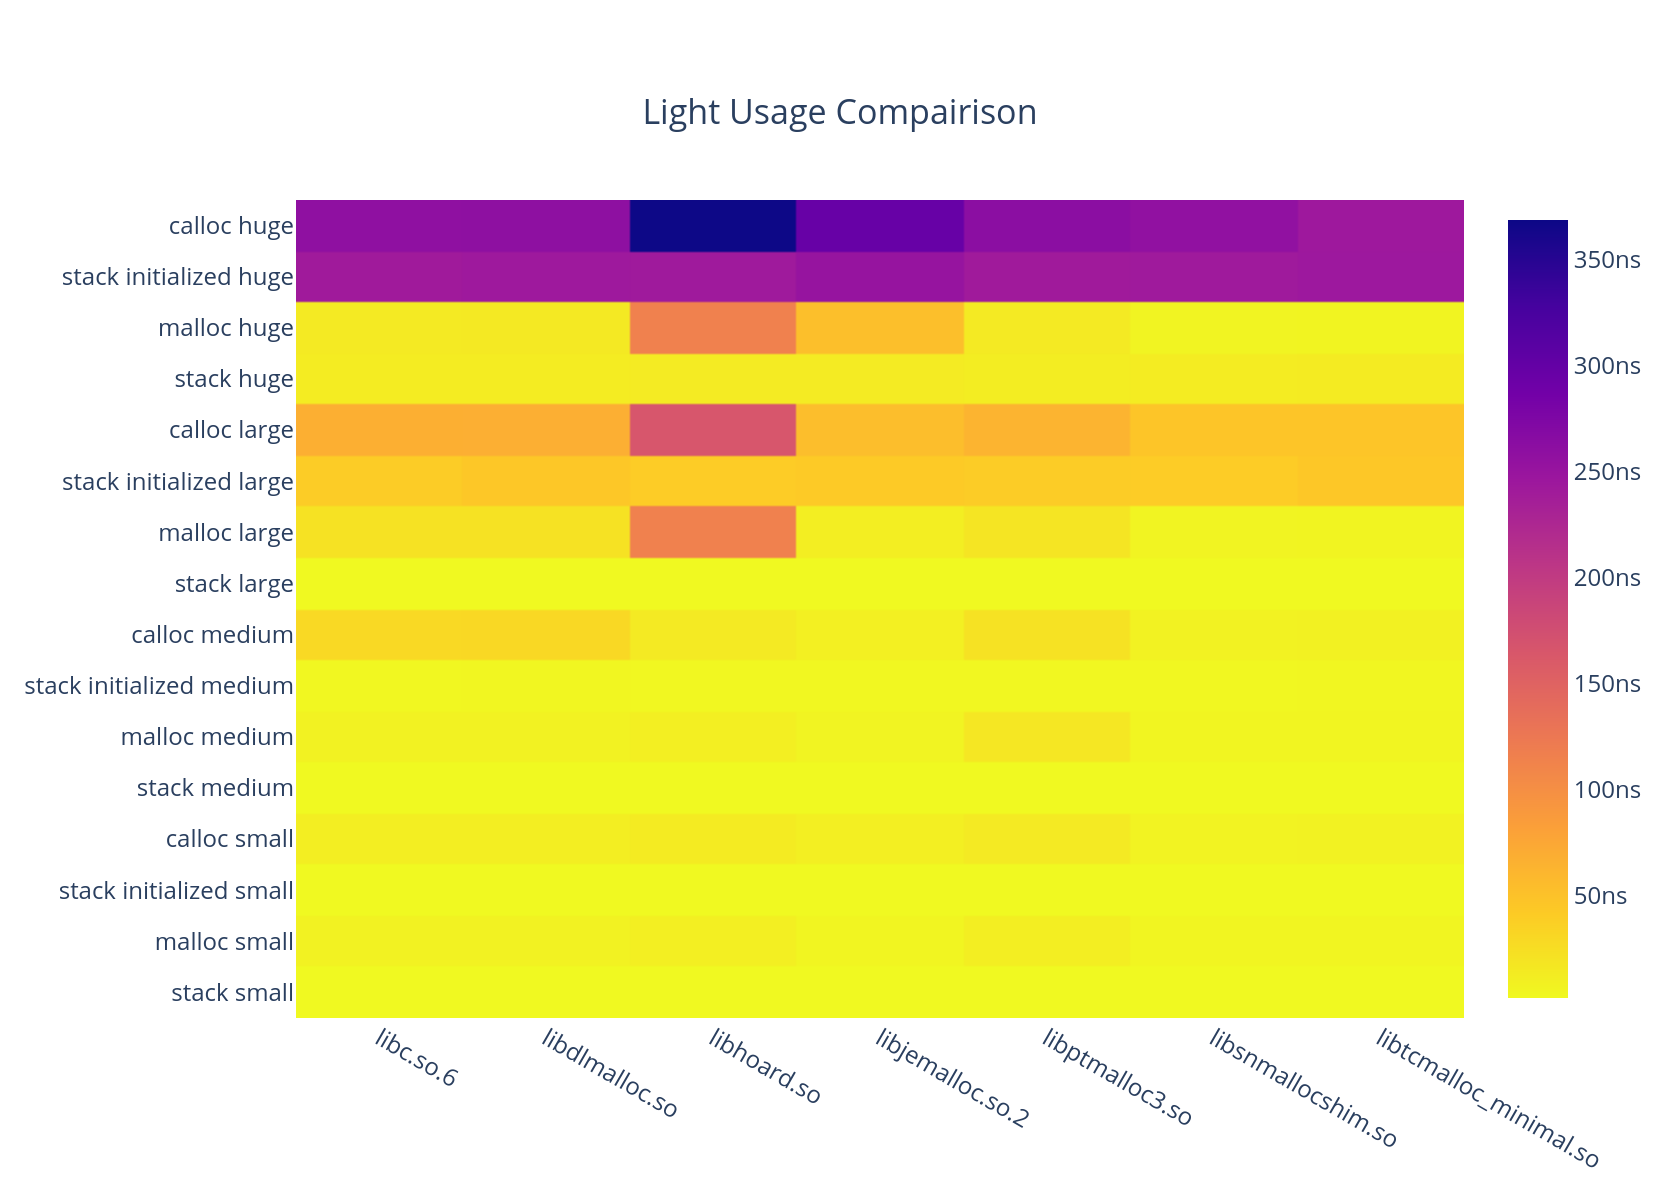
\includegraphics[width=\columnwidth]{graphs/light_hist.png}
  \caption{ Comparison of allocation methods in nano seconds }
  \label{algo1_complete_hist}
\end{figure} 


Fig. \ref{algo1_libc.so.6_bar} shows a better comparison of allocation times by organizing the results of a single library by allocation size.
From the speed comparison for libc.so.6, it becomes evident that calloc is generally the slowest and normal stack allocation is a constant speed across all allocation sizes.
This figure also shows the progressive time increases that both calloc and initialized stack allocations go through as the allocation size increases.
It should also be noted that malloc and uninitialized stack allocations have relatively fixed performance costs, despite a small speed decrease in malloc when the size changes from medium to large.

\begin{figure}[tbh!]
  \centering
  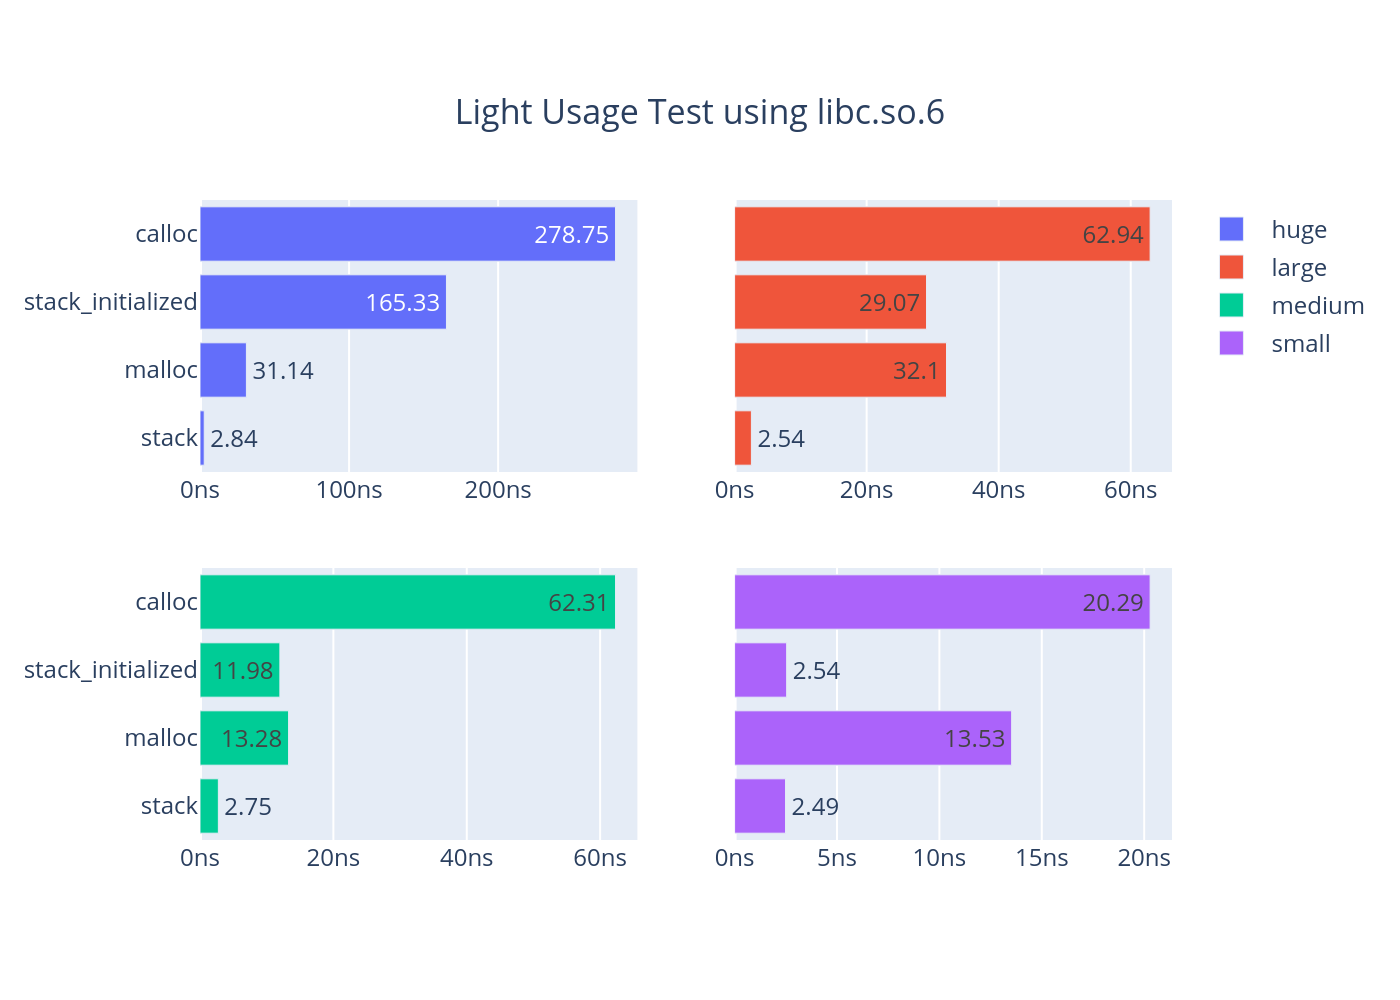
\includegraphics[width=\columnwidth]{{graphs/light_libc.so.6_1s_20}.png} %stupid .'s in file names
  \caption{ Performance differences in libc.so.6 between allocation methods at various sizes }
  \label{algo1_libc.so.6_bar}
\end{figure} 

Algorithm \ref{light_usage_algorithm} has consistent performance across all allocation sizes when allocating on the stack.
Fig. \ref{algo1_stack_malloc_hist} shows a relative comparison between stack allocation and the efficiency of malloc.
From this figure, the performance of malloc across allocation libraries is shown to vary greatly depending on the size of the allocation.
For most allocation libraries, the difference in performance between stack and malloc allocation is minimal, however some allocation libraries.

The main reason for the relatively constant allocation times for malloc is due to the performance improvements that the allocation libraries implemented.
Most allocation libraries implement chunk bins in some fashion.\footnote{\href{https://sourceware.org/glibc/wiki/MallocInternals\#Arenas\_and\_Heaps}{glibc heap bin explanation}}
Use of bins keeps allocation times relatively constant since previously allocated chunks can be easily retrieved from a bin without needed to go through the full allocaiton process.

\begin{figure}[tbh!]
  \centering
  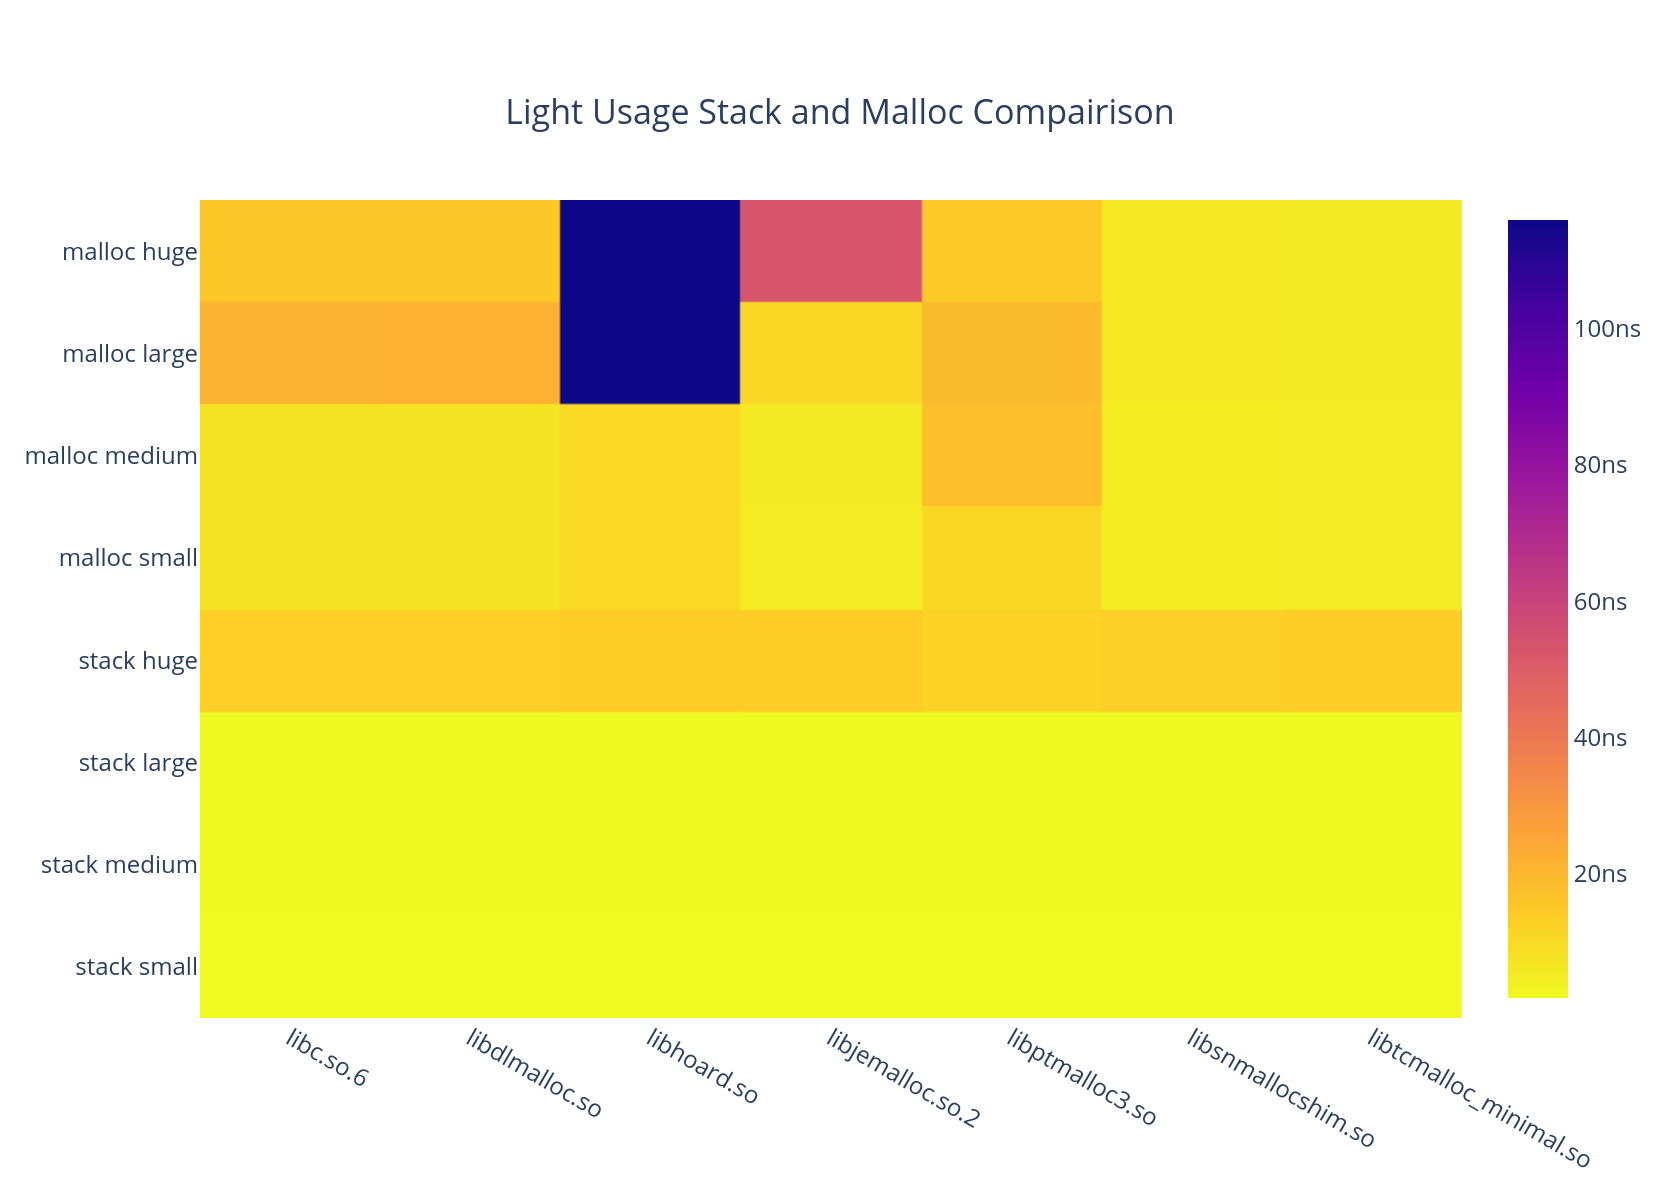
\includegraphics[width=\columnwidth]{graphs/light_stack_malloc_hist.png}
  \caption{ Stack and Malloc execution times using Algo. \ref{light_usage_algorithm} } 
  \label{algo1_stack_malloc_hist}
\end{figure}

The difference in performance between initialization stack allocation and calloc is the time of uninitialized allocation plus the cost of initialization.
However, looking at Fig. \ref{algo1_libc.so.6_bar} initialized stack allocation does not appear to be following this rule.
This is due to the compiler optimizations which perform loop unwinding during initialization of the stack.
Loop unwinding for reasonably small allocations can be performed with a store of $0$ using an MMX register or other sufficiently large register.
This is what allows initialized stack allocation for small allocations to perform on par with uninitialized stack allocaitons in the small allocaiton tests.

Applying the idea of loop unwinding to calloc however does not work, as see in Fig. \ref{algo1_init_calloc_hist}.
Since calloc is an external library, it is unable to benefit from the compiler optimizations that the initialized stack allocaiton does.
The main reason for this is that calloc is written in such a way so as to allow for general purpose allocaiton, and can therefore accommodate any size of allocation with a single function.
Loop unwinding requires knowledge of the size of the allocation so as to unwind the appropriate number of times without overrunning or underrunning the buffer. 

\begin{figure}[tbh!]
  \centering
  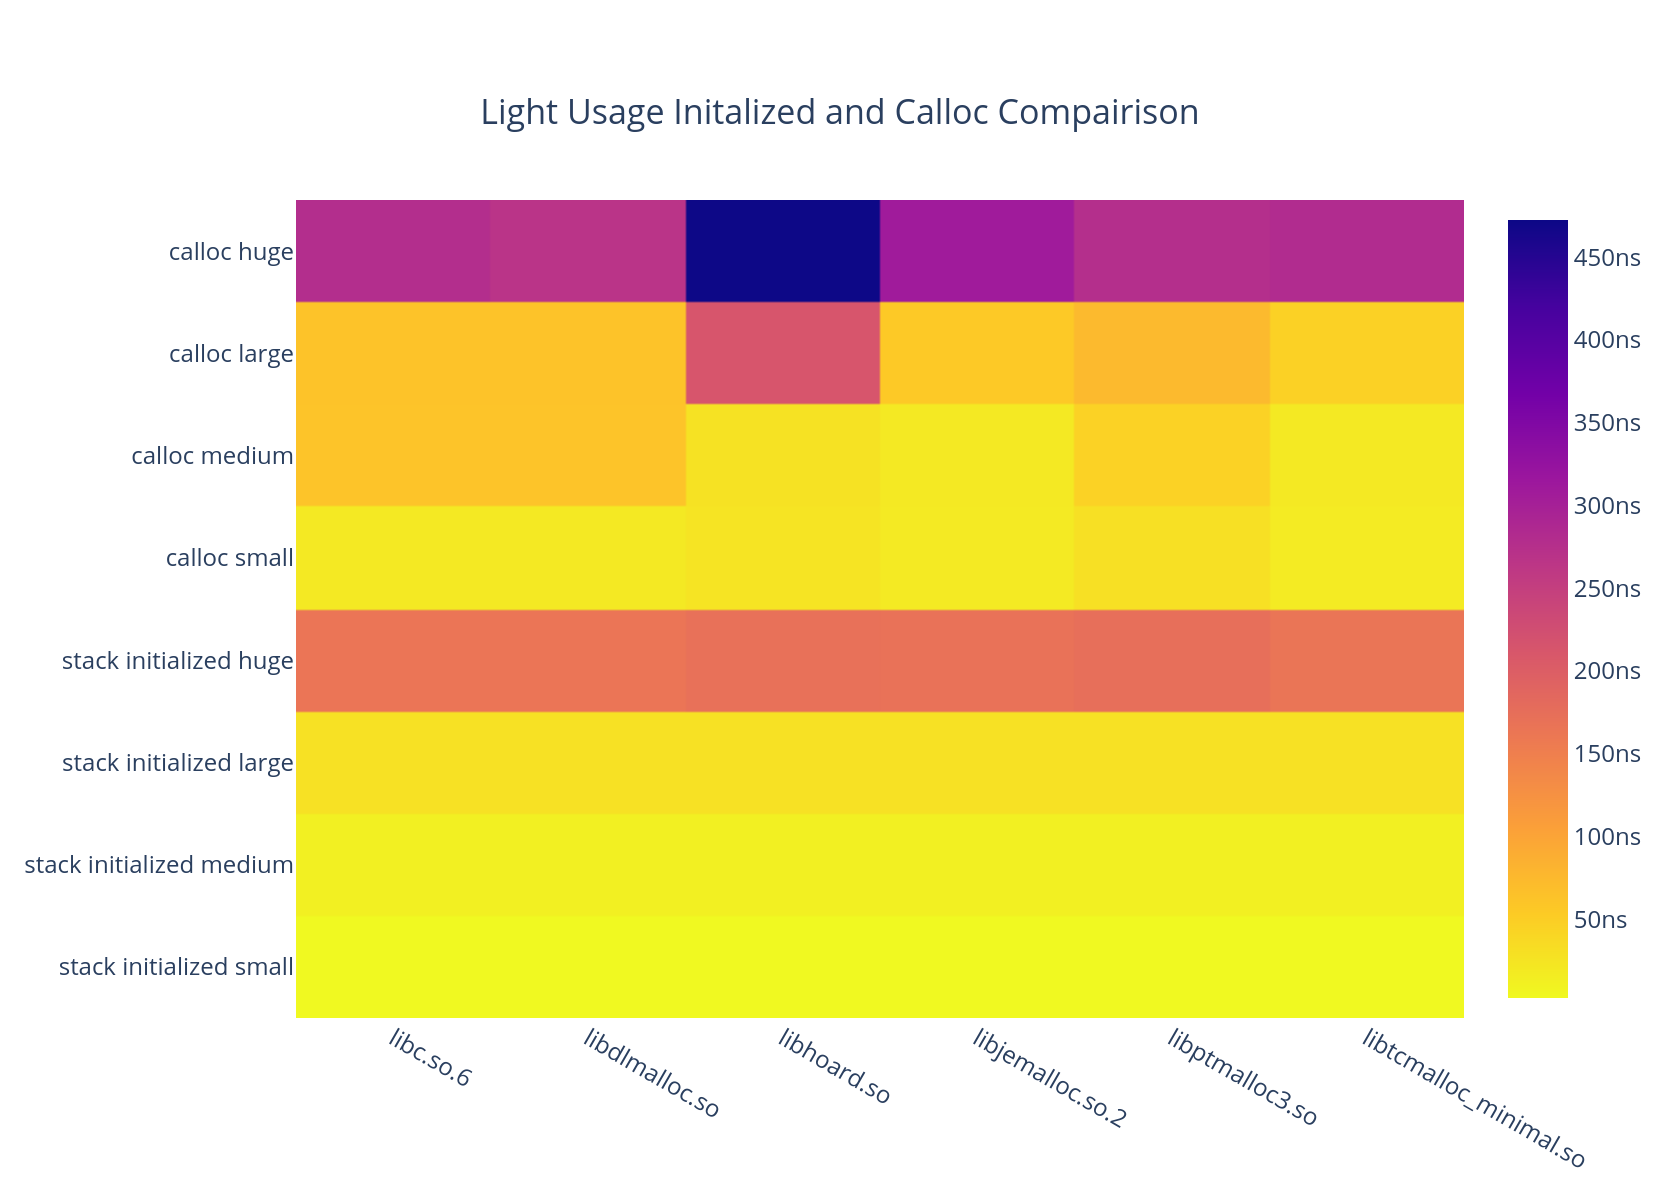
\includegraphics[width=\columnwidth]{graphs/light_init_calloc_hist.png}
  \caption{ Initialized Stack and Calloc execution times using Algo. \ref{light_usage_algorithm} }
  \label{algo1_init_calloc_hist}
\end{figure} 

Taking a look at performance in a multithreaded environment, Fig. \ref{algo1_stack_malloc_threaded_hist} shows how stack and malloc allocaitons perform.

\todo \url{https://sourceware.org/glibc/wiki/MallocInternals#Thread_Local_Cache_.28tcache.29}

\begin{figure}[tbh!]
  \centering
  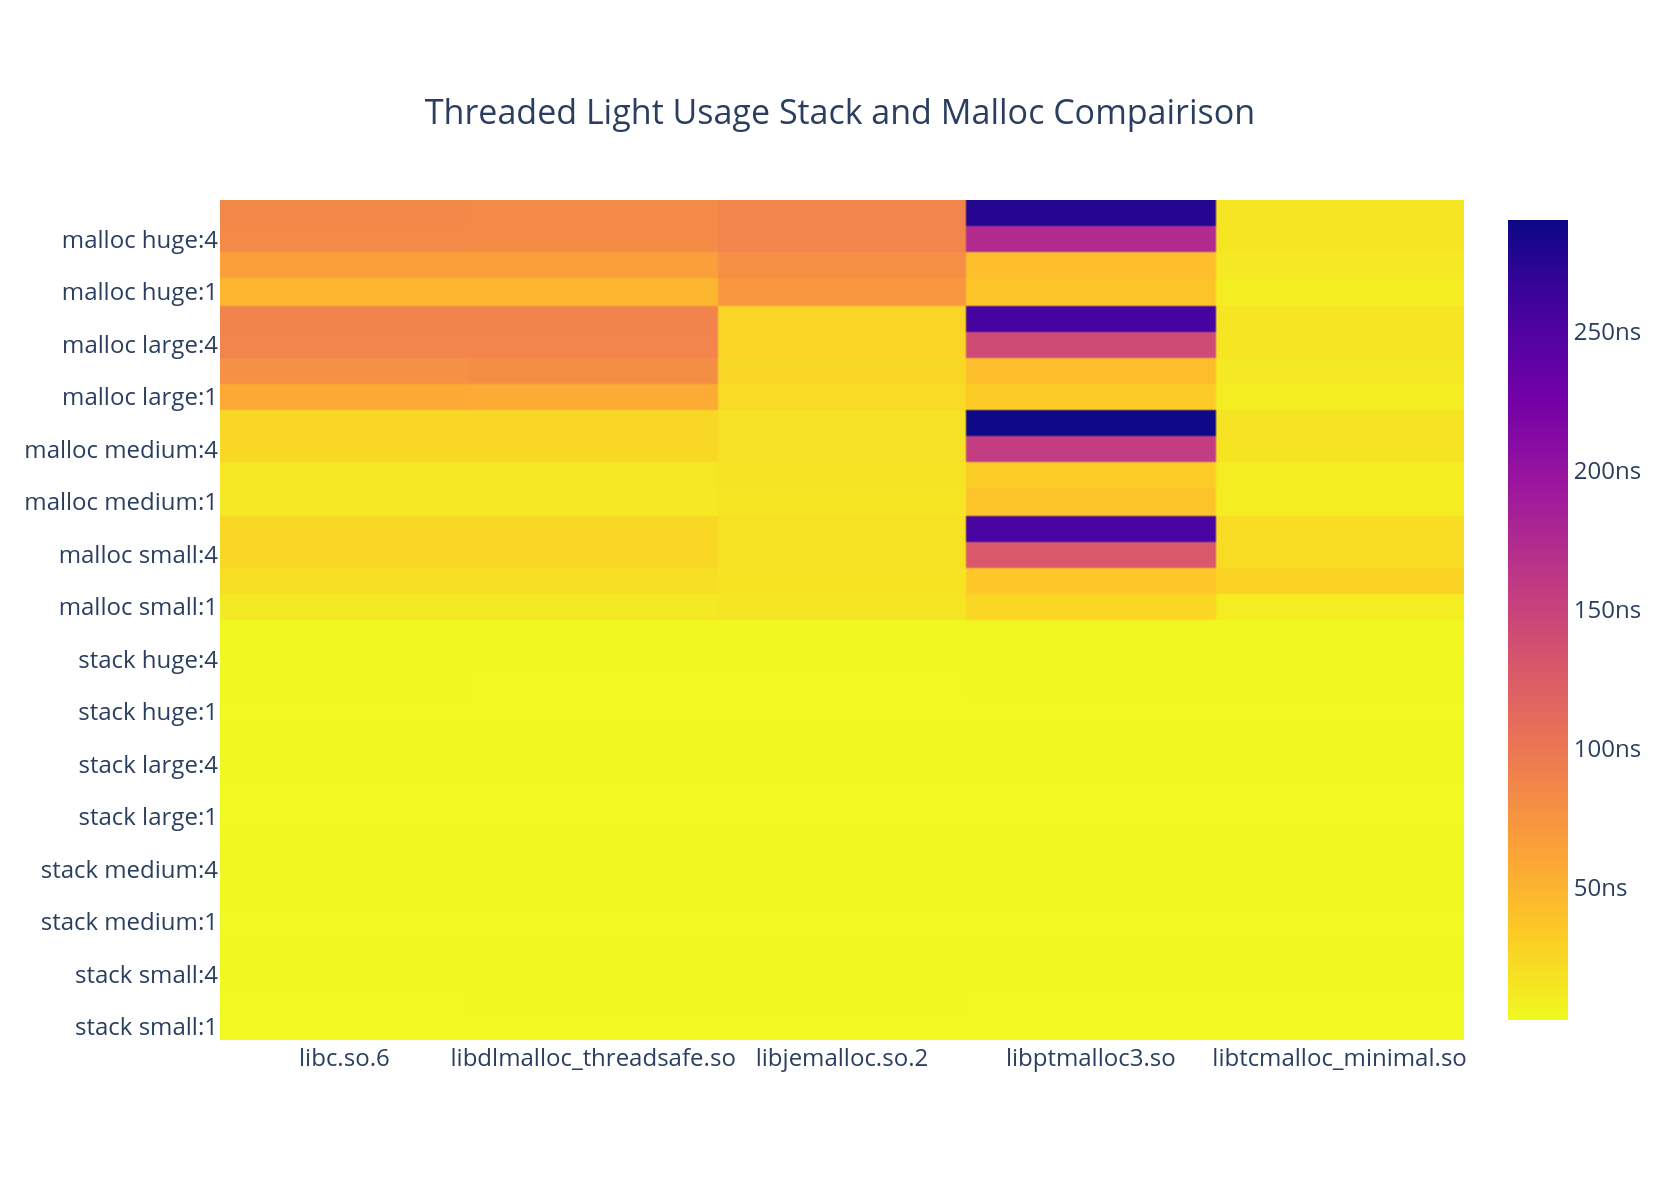
\includegraphics[width=\columnwidth]{graphs/light_stack_malloc_threaded_hist.png}
  \caption{ Comparison of stack and malloc allocations during multithreaded execution }
  \label{algo1_stack_malloc_threaded_hist}
\end{figure}

\begin{figure}[tbh!]
  \centering
  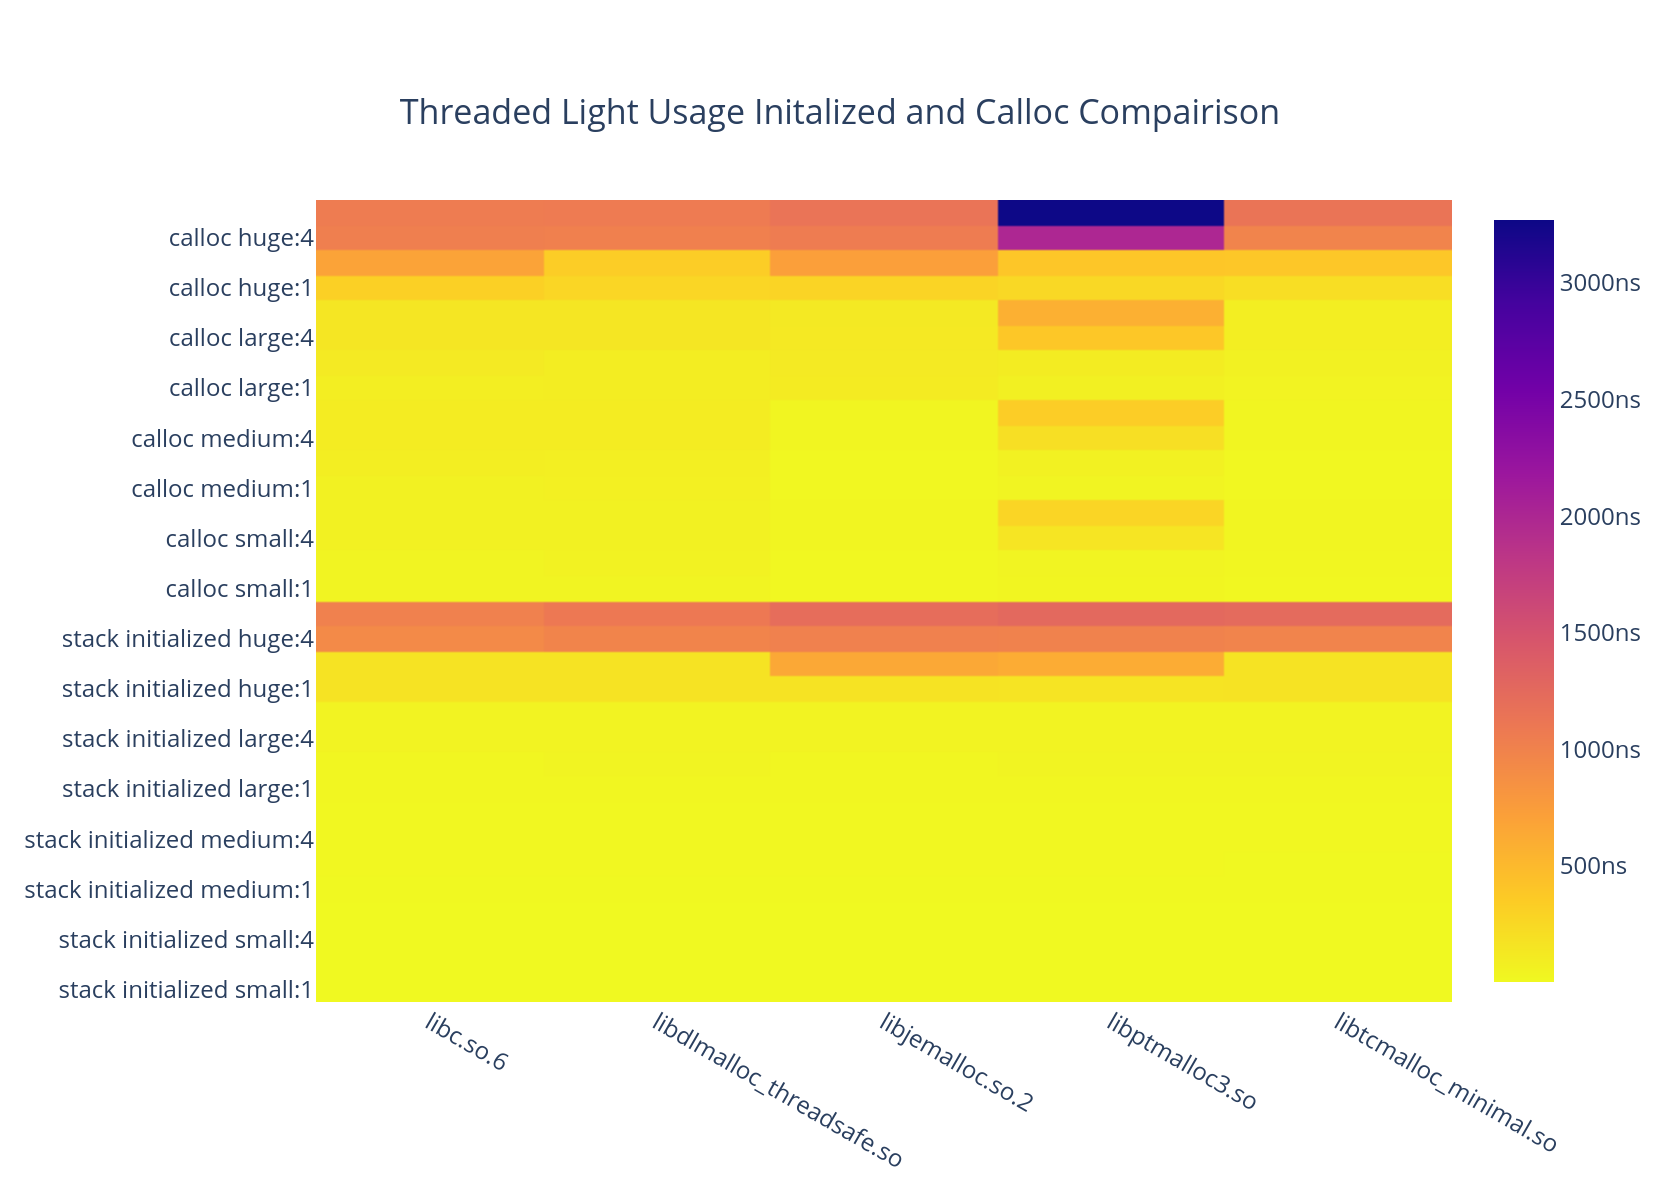
\includegraphics[width=\columnwidth]{graphs/light_init_calloc_threaded_hist.png}
  \caption{ \todo }
  \label{algo1_init_calloc_threaded_hist}
\end{figure}

%%%%%%%%%%%%%%%%%%%%%%%%%%%%%%%%%%%%%%%%%%%%%%%%%%%%%%%%%%%%%%%%%%%%%%%%%%%%%%%%
\section{Experiment: Algorithm \ref{struct_usage_algorithm}}

\todo talk about the overall results in this section referencing Fig. \ref{algo2_complete_hist}

\begin{figure}[tbh!]
  \centering
  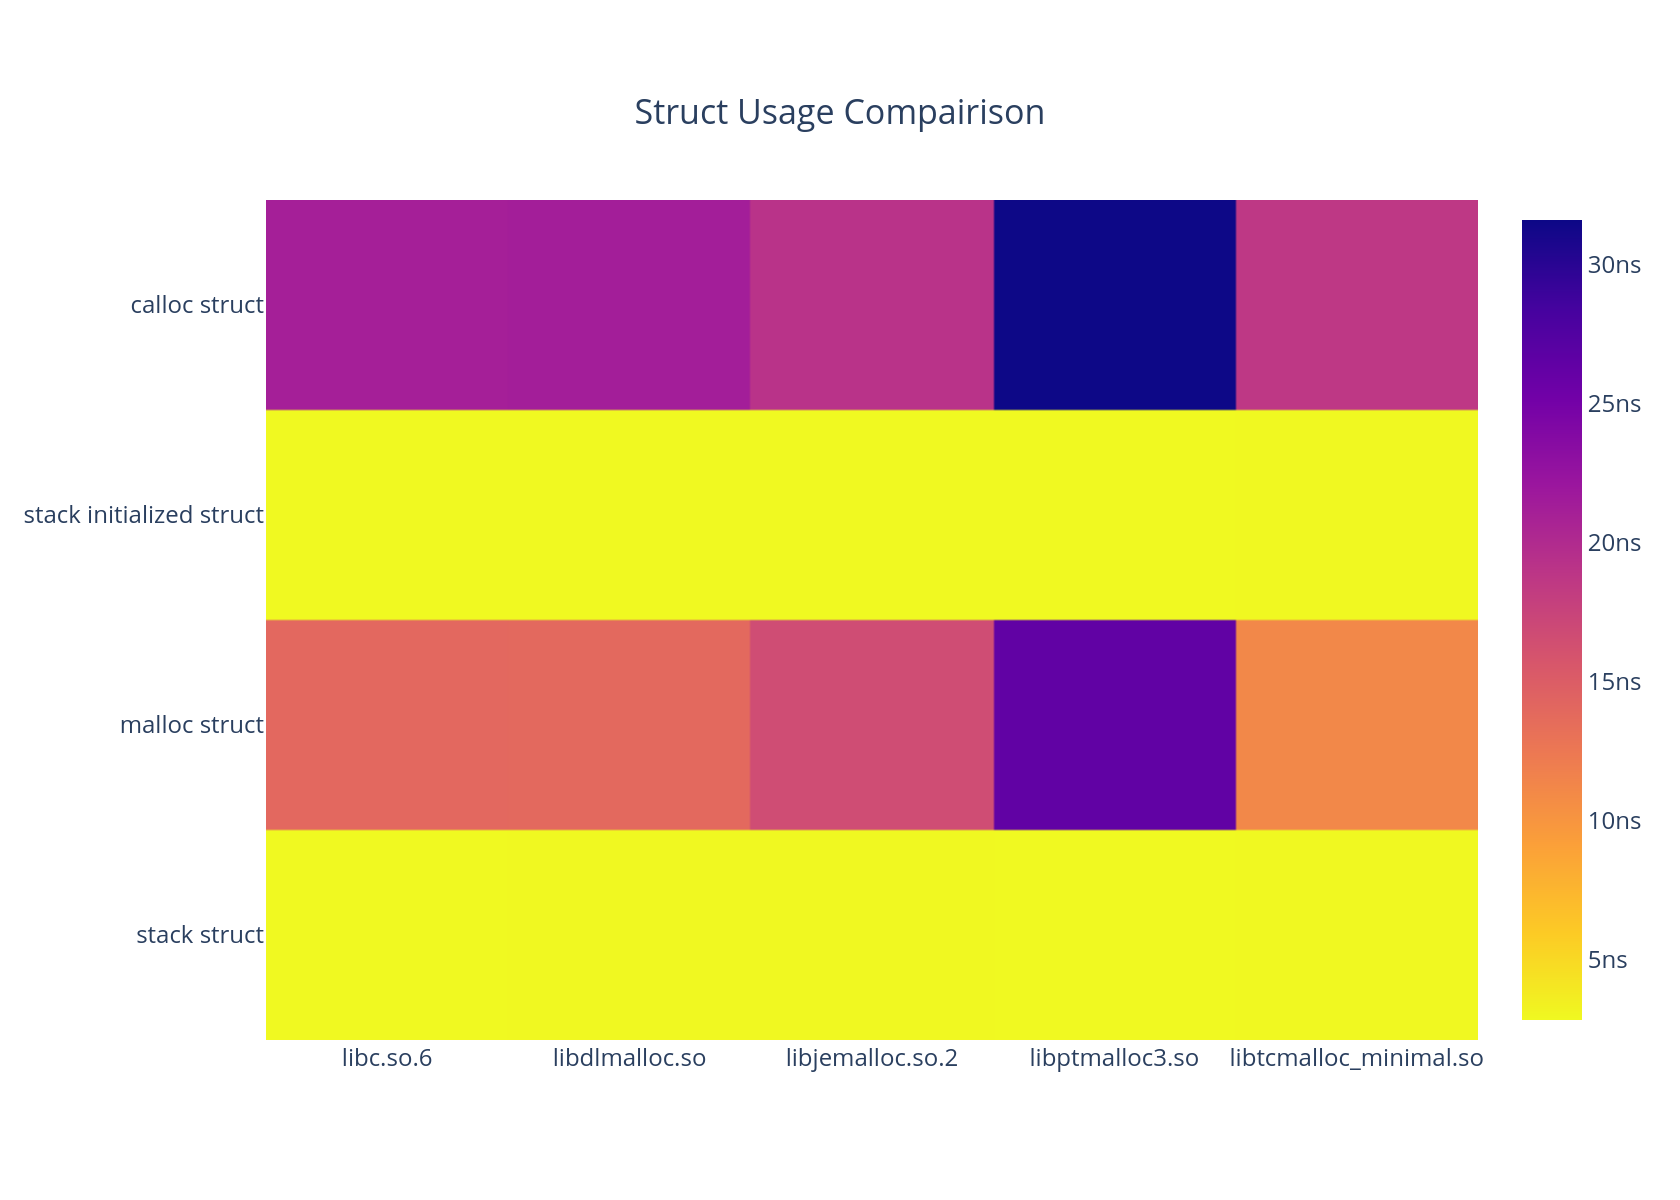
\includegraphics[width=\columnwidth]{graphs/struct_hist.png}
  \caption{ Comparison of allocation methods in nano seconds }
  \label{algo2_complete_hist}
\end{figure} 

\todo Fig. \ref{algo2_complete_threaded_hist}

\begin{figure}[tbh!]
  \centering
  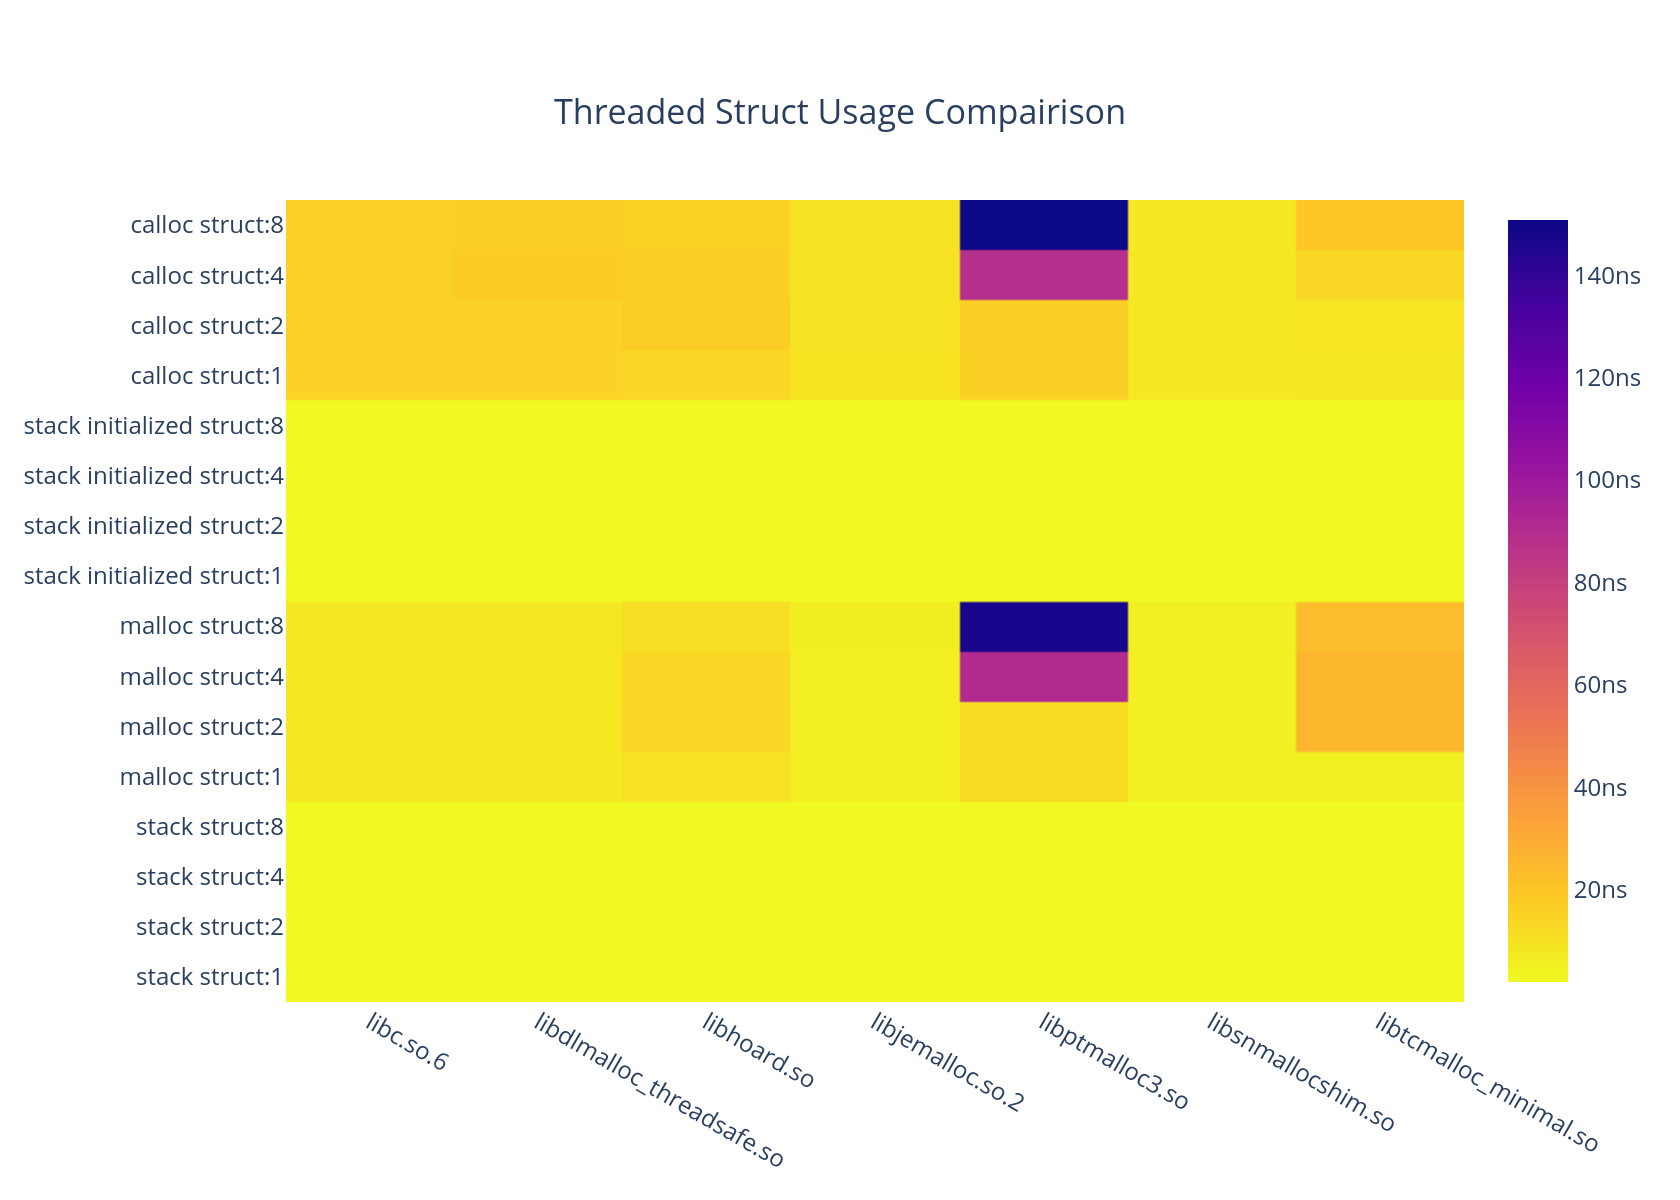
\includegraphics[width=\columnwidth]{graphs/struct_threaded_hist.png}
  \caption{ \todo  test}
  \label{algo2_complete_threaded_hist}
\end{figure}

\todo talk about how stack and malloc compare in Fig. \ref{algo2_stack_malloc_hist}.

\begin{figure}[tbh!]
  \centering
  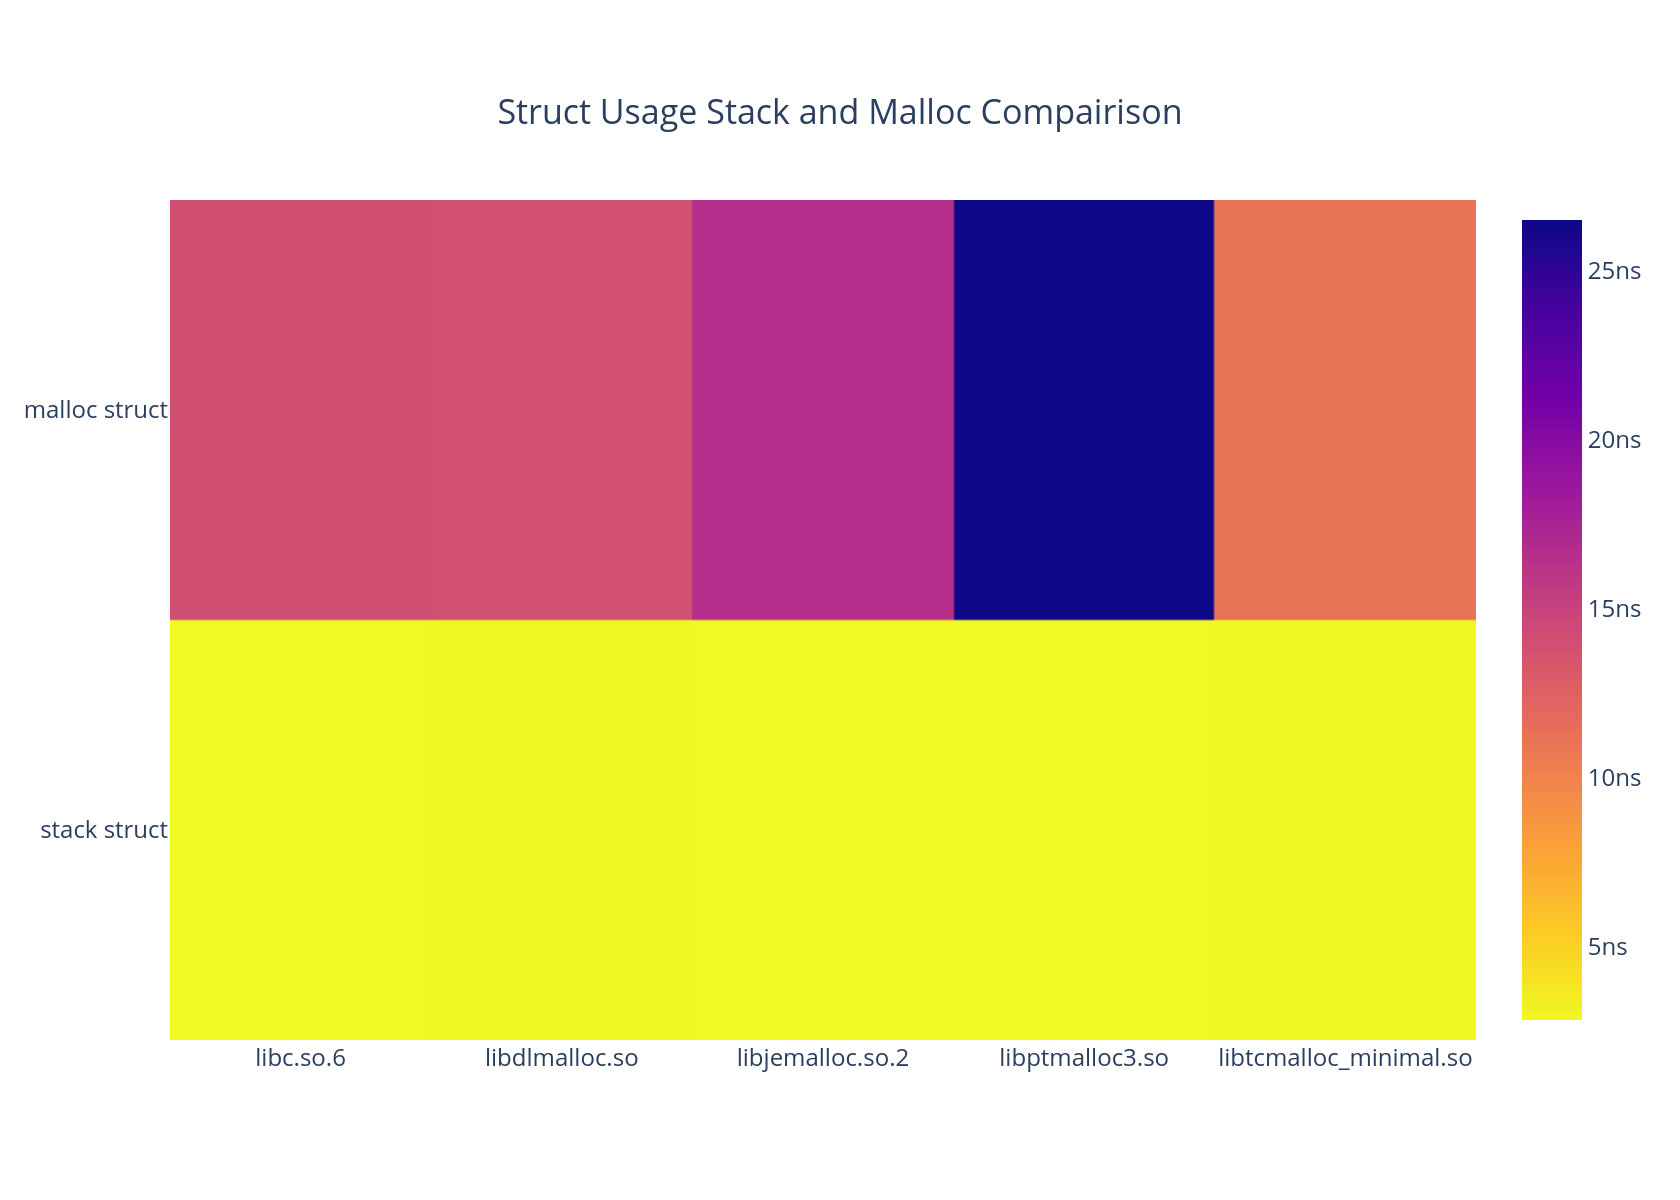
\includegraphics[width=\columnwidth]{graphs/struct_stack_malloc_hist.png}
  \caption{ \todo Should this be a bar graph? }
  \label{algo2_stack_malloc_hist}
\end{figure}

\todo talk about why calloc is so much slower then initalized stack in Fig. \ref{algo2_init_calloc_hist}.

\begin{figure}[tbh!]
  \centering
  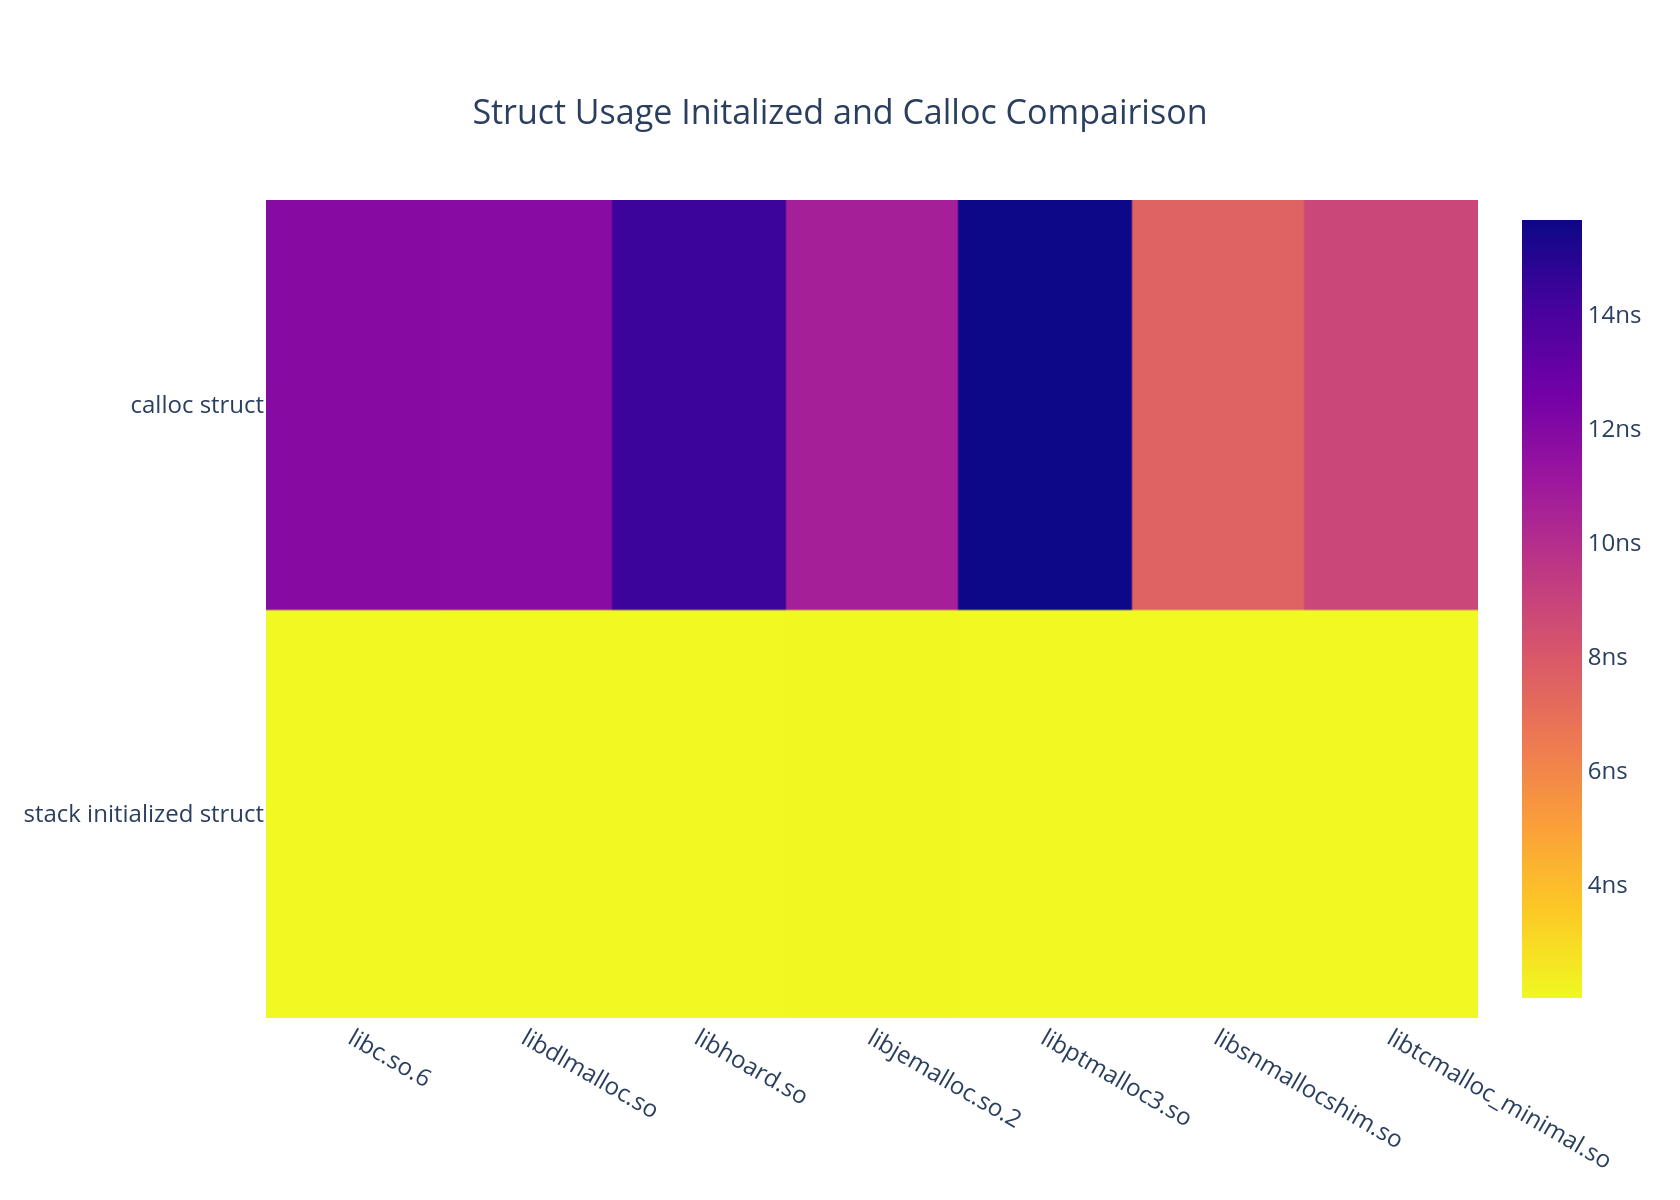
\includegraphics[width=\columnwidth]{graphs/struct_init_calloc_hist.png}
  \caption{ \todo Should this be a bar graph? }
  \label{algo2_init_calloc_hist}
\end{figure} 

%%%%%%%%%%%%%%%%%%%%%%%%%%%%%%%%%%%%%%%%%%%%%%%%%%%%%%%%%%%%%%%%%%%%%%%%%%%%%%%%
\section{Experiment: Algorithm \ref{network_usage_algorithm}}

\todo Fig. \ref{algo3_complete_hist}

\begin{figure}[tbh!]
  \centering
  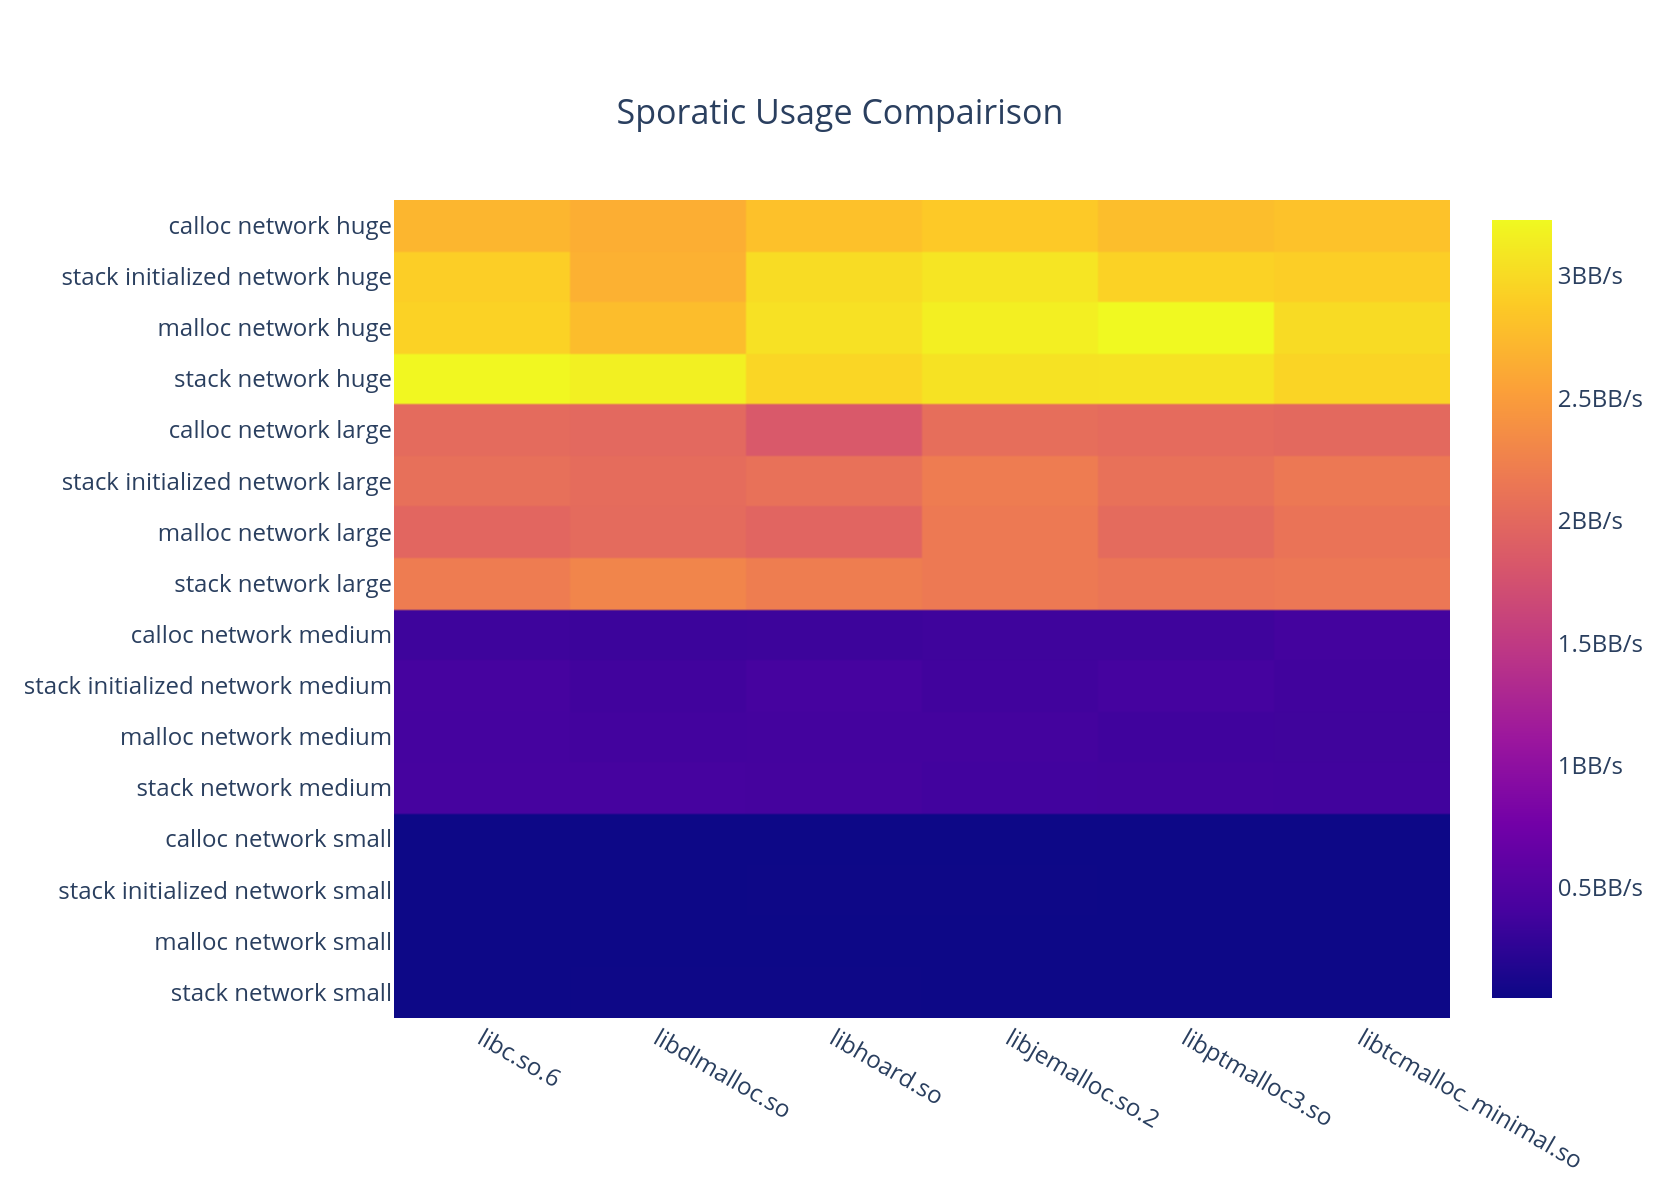
\includegraphics[width=\columnwidth]{graphs/sporatic_hist.png}
  \caption{ \todo }
  \label{algo3_complete_hist}
\end{figure}

\todo Fig. \ref{algo3_complete_threaded_hist}

\begin{figure}[tbh!]
  \centering
  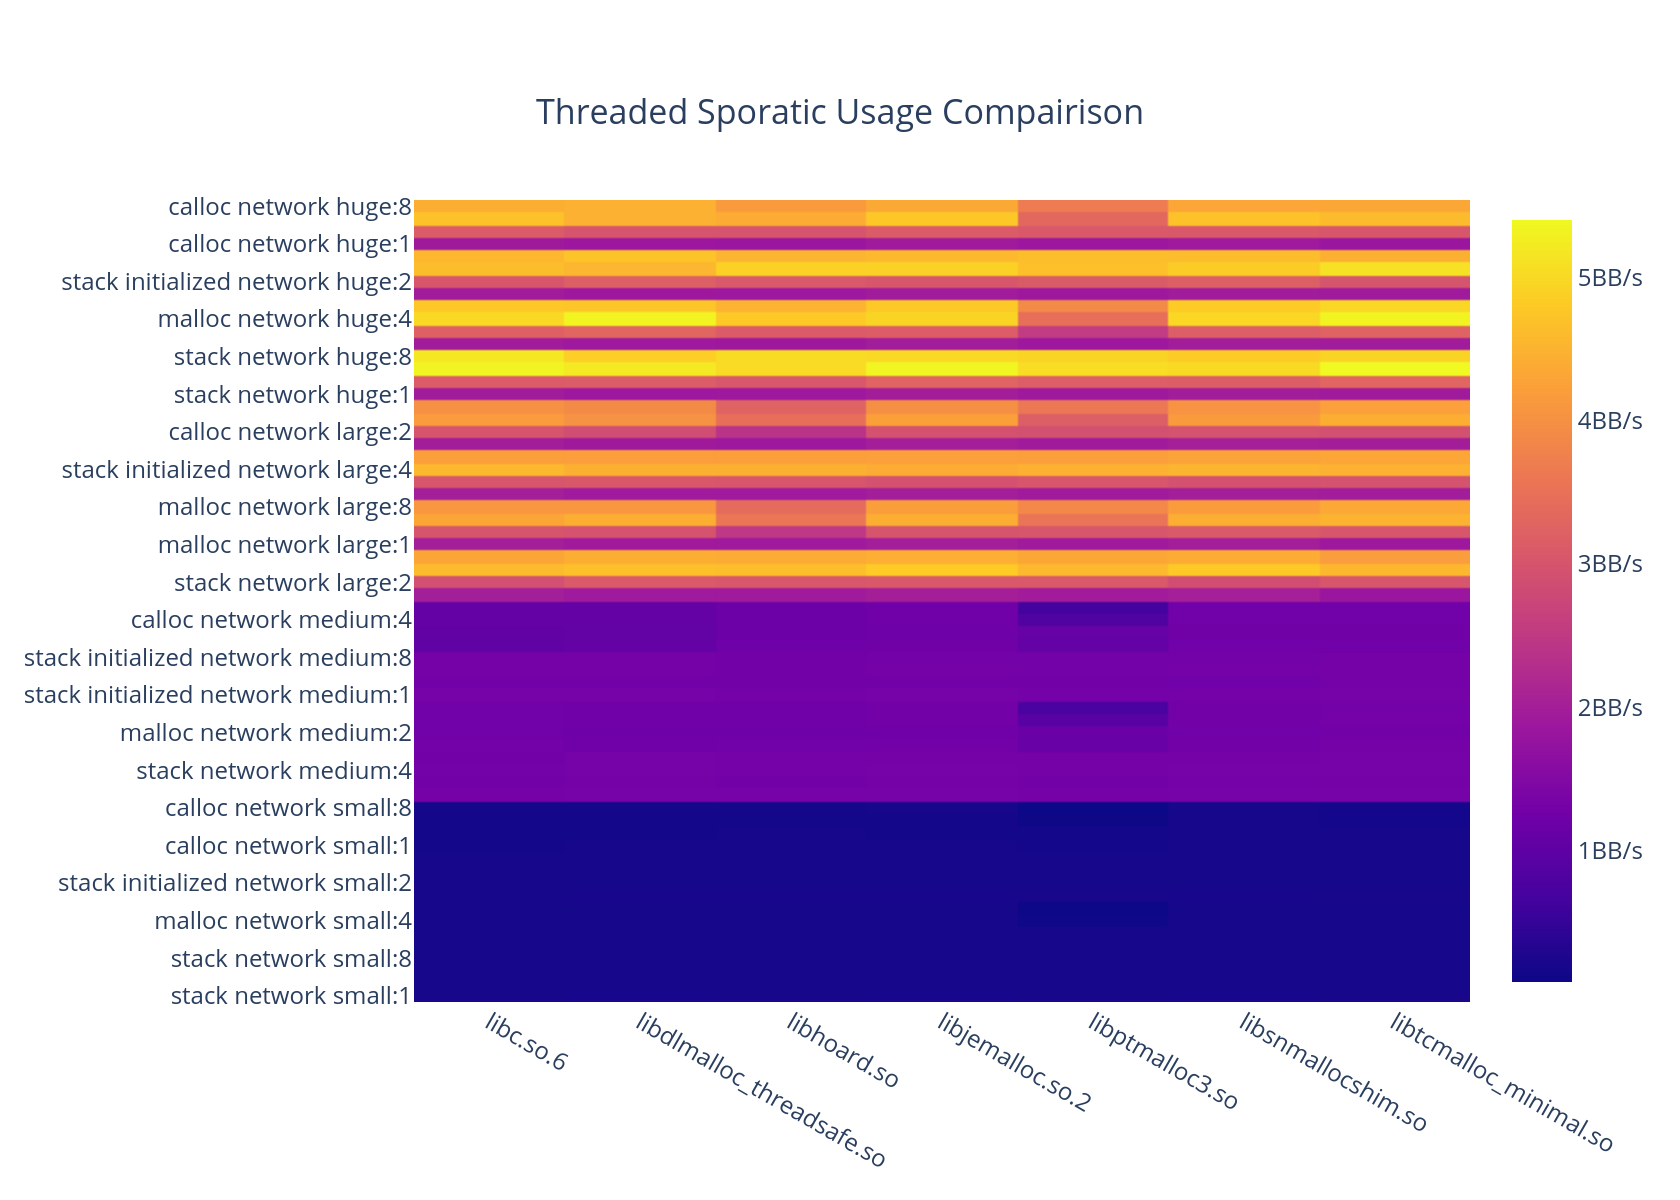
\includegraphics[width=\columnwidth]{graphs/sporatic_threaded_hist.png}
  \caption{ \todo }
  \label{algo3_complete_threaded_hist}
\end{figure}


\todo Fig. \ref{algo3_stack_malloc_hist}

\begin{figure}[tbh!]
  \centering
  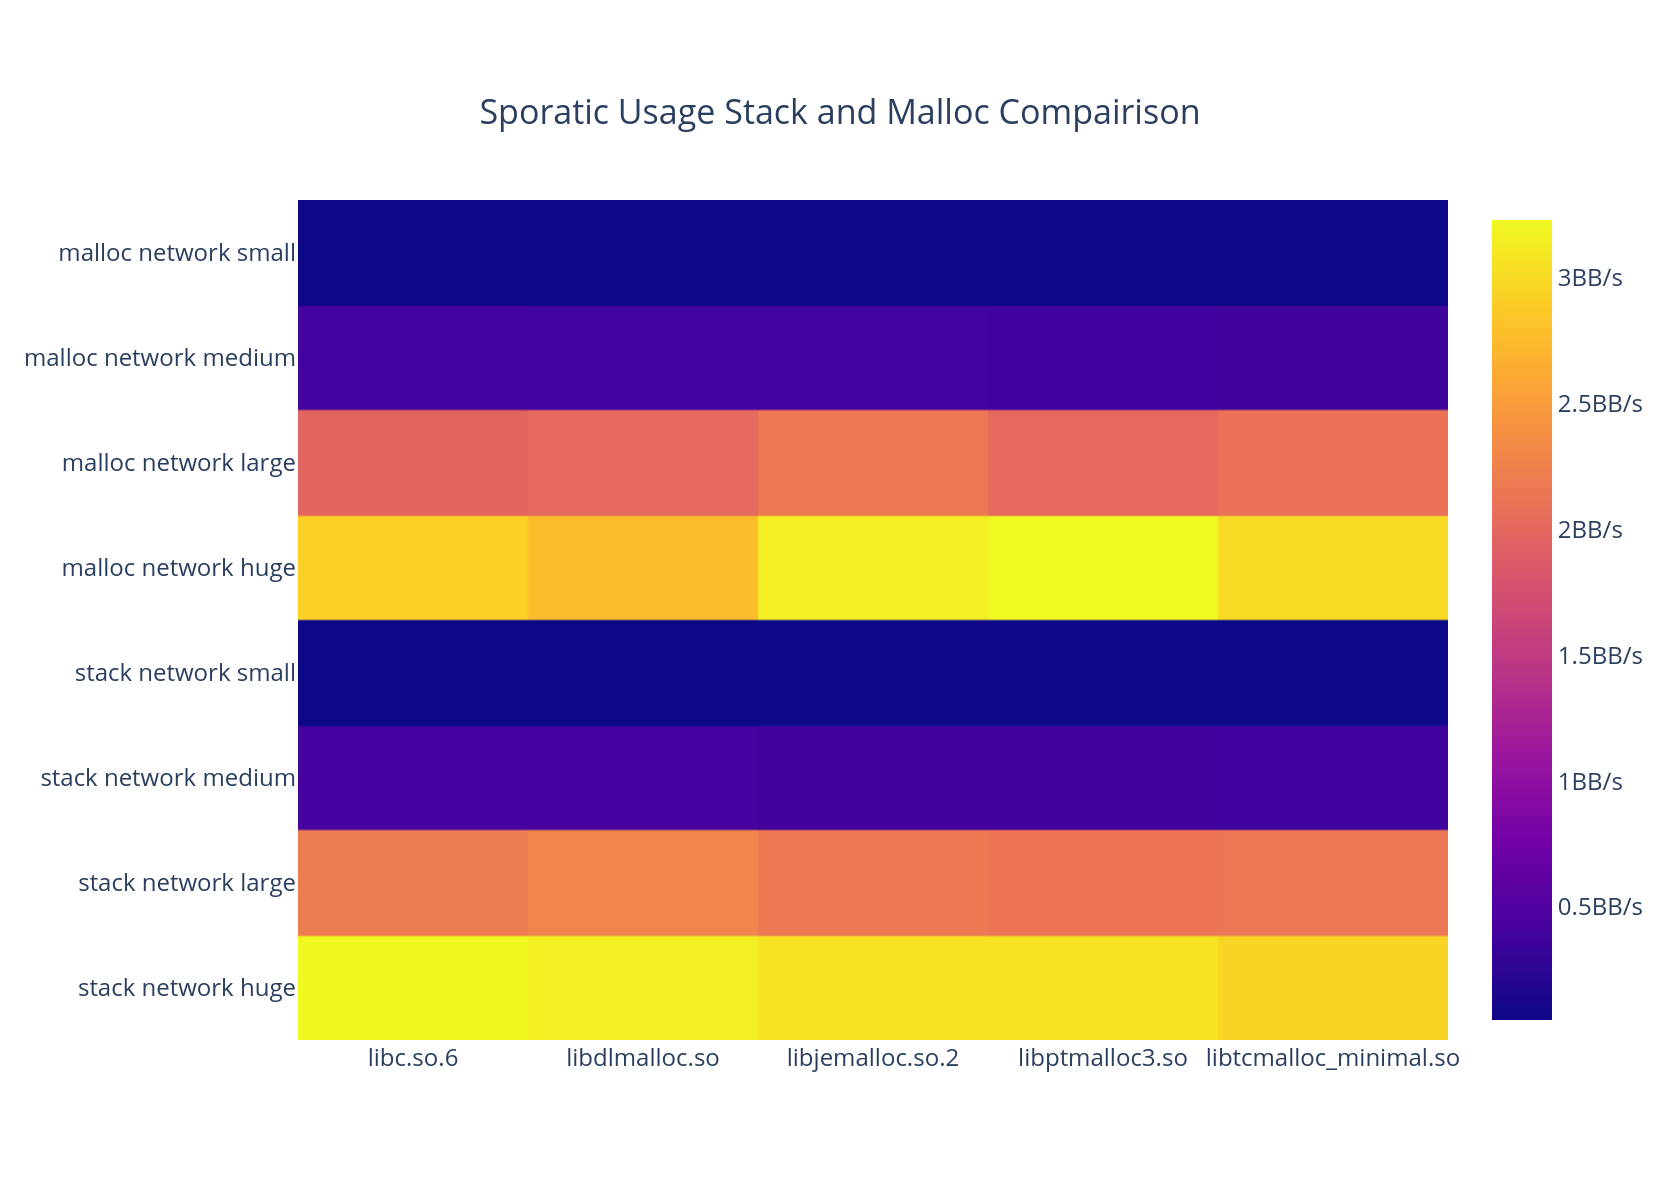
\includegraphics[width=\columnwidth]{graphs/sporatic_stack_malloc_hist.png}
  \caption{ \todo }
  \label{algo3_stack_malloc_hist}
\end{figure}

\todo Fig. \ref{algo3_init_calloc_hist}

\begin{figure}[tbh!]
  \centering
  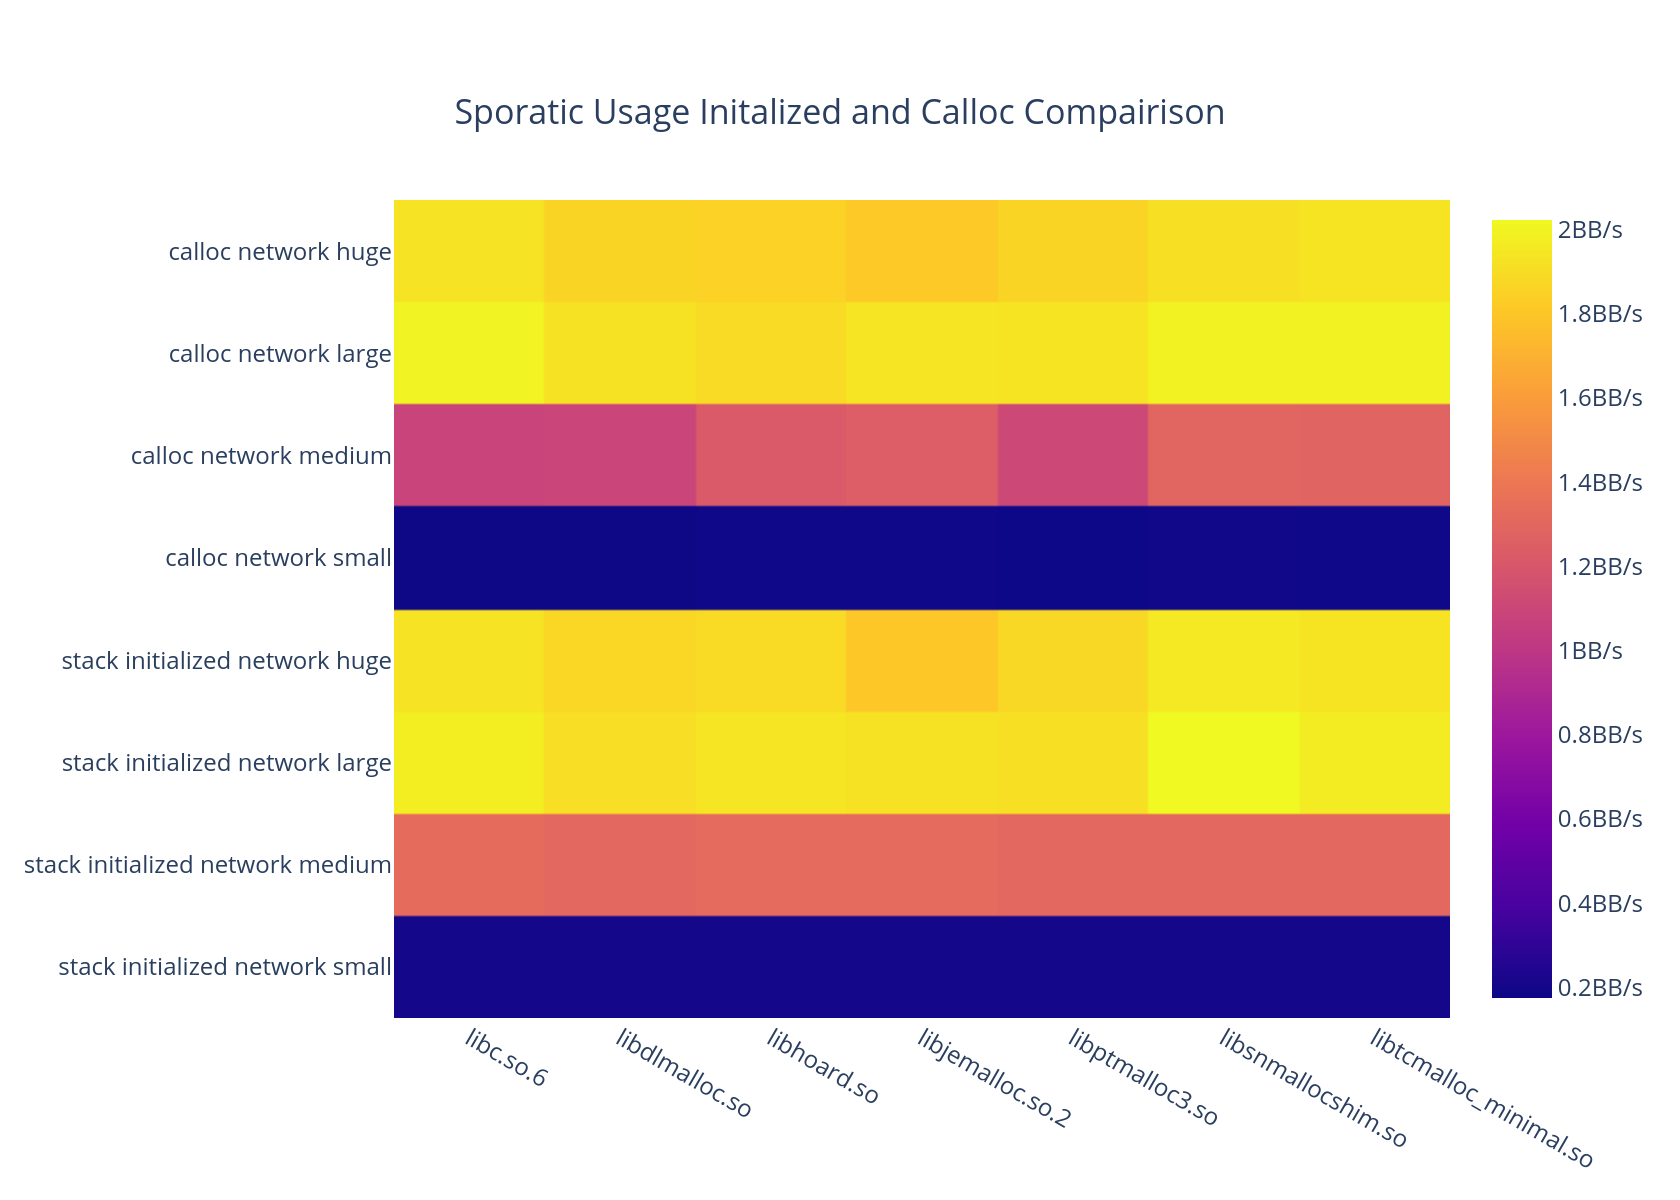
\includegraphics[width=\columnwidth]{graphs/sporatic_init_calloc_hist.png}
  \caption{ \todo }
  \label{algo3_init_calloc_hist}
\end{figure}

%%%%%%%%%%%%%%%%%%%%%%%%%%%%%%%%%%%%%%%%%%%%%%%%%%%%%%%%%%%%%%%%%%%%%%%%%%%%%%%%
\section{Discussion}


%%%%%%%%%%%%%%%%%%%%%%%%%%%%%%%%%%%%%%%%%%%%%%%%%%%%%%%%%%%%%%%%%%%%%%%%%%%%%%%%
\section{Conclusions}

%%%%%%%%%%%%%%%%%%%%%%%%%%%%%%%%%%%%%%%%%%%%%%%%%%%%%%%%%%%%%%%%%%%%%%%%%%%%%%%%
\section{Source Code}

Source code for all experiments detailed in this paper can be found at \url{\GitHubLoc}.

%%%%%%%%%%%%%%%%%%%%%%%%%%%%%%%%%%%%%%%%%%%%%%%%%%%%%%%%%%%%%%%%%%%%%%%%%%%%%%%%
\section{Additional Figures}

% \begin{figure}[tbp]
% \centering
% \includegraphics[width=\columnwidth]{figure_1.png}
% \caption{blah }
% \label{loss_spikes}
% \end{figure}

%%%%%%%%%%%%%%%%%%%%%%%%%%%%%%%%%%%%%%%%%%%%%%%%%%%%%%%%%%%%%%%%%%%%%%%%%%%%%%%%
\section{Acknowledgements}

\noindent This research was funded by .

\clearpage

\end{document}
